\subsection{Preliminary Iteration: WebXR Drone Physics Implementation}

\paragraph{Design}

In the initial design iteration, the implementation of drone physics was simplified. Unlike full physical modeling of multi-rotor dynamics, including clockwise (CW) and counter-clockwise (CCW) torque balancing as described in \cref{eq:torque}, the first prototype adopted a simplified physics representation.

The drone object was implemented in the Wonderland Engine using the PhysX system provided by NVIDIA. A box collider was used as the primary collision shape, ensuring basic physical interaction with the environment. The system included two primary state variables: appliedForce and appliedTorque, which were updated in each frame within the update loop. User input was processed through a custom ReadInput function that retrieved joystick values from the WebXR input API, due to the lack of native input profile configuration support in the Wonderland Engine. The drone object design is illustrated in \cref{fig:webxr_drone}.

\begin{figure}[H]
    \caption{Components of the drone Object}\label{fig:webxr_drone}
    \centering
\begin{tikzpicture}

\umlclass[x=0, y=0]{DroneObject}{
  - appliedForce : float \\
  - appliedTorqueYaw : float \\
  - appliedTorqueRoll: float \\
  - appliedTorquePitch: float \\
  \dots
}{
  + Update() : void \\
  + ReadInput() : void
}

\umlclass[x=6, y=2]{PhysXComponent}{
  + shape : Box \\
  + engine : NVIDIA PhysX
}{
}

\umlclass[x=6, y=-2]{CollisionComponent}{
      + shape : Box 
}{
}

\umluniassoc{DroneObject}{PhysXComponent}
\umluniassoc{DroneObject}{CollisionComponent}

\end{tikzpicture}
\end{figure}


\paragraph{Enactment}

During implementation, the system was able to run in a WebXR environment; however, unstable flight behavior was observed. In particular, the drone exhibited oscillatory motion during navigation, and the tuning of applied torque parameters did not produce consistent control behavior.

\begin{figure}[H]
    \caption{Preliminary implementation of drone physics in WebXR}\label{fig:webxr}
    \centering
    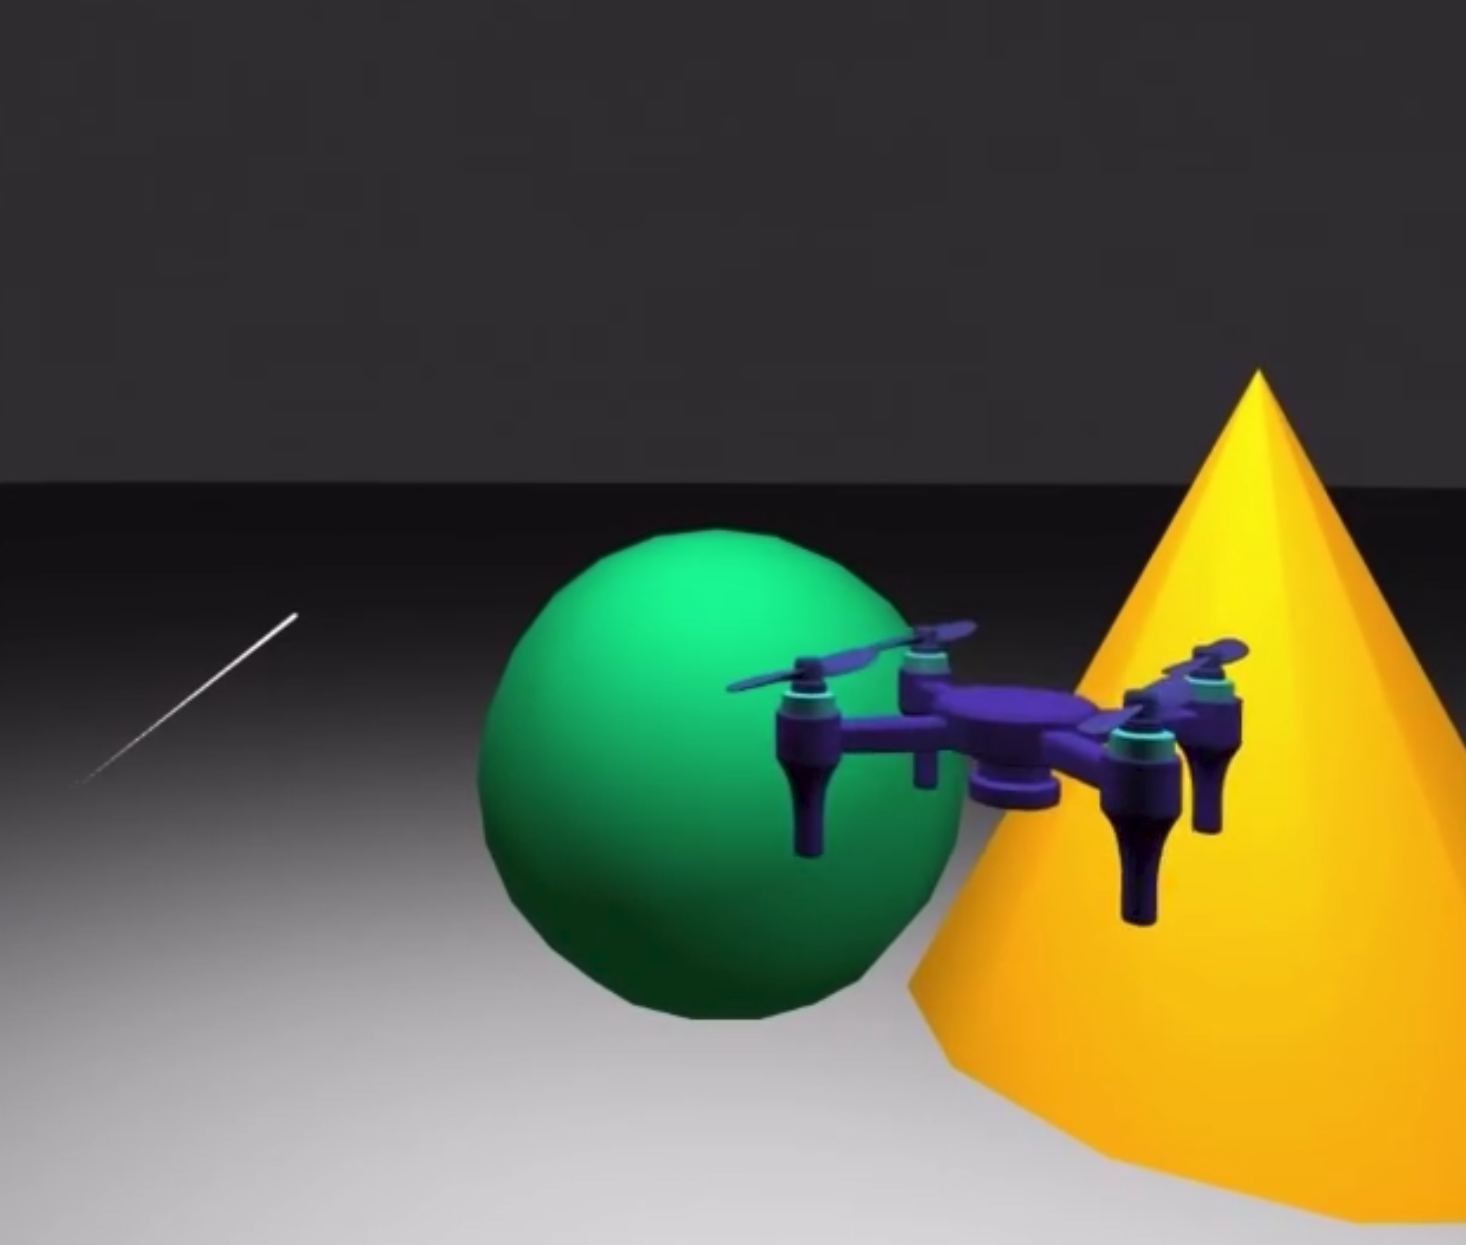
\includegraphics[width=0.6\linewidth]{img/webxr.png}
\end{figure}

The cause of these issues could not be conclusively identified within this iteration. Potential factors include limitations in browser-based physics execution, instability in the WebXR runtime environment, or insufficient documentation and debugging support in the Wonderland Engine.

As a result, alternative development platforms were explored. Microsoft AirSim \parencite{shah_airsim_2017}, built on Unreal Engine, was initially considered due to its advanced simulation capabilities. However, hardware constraints on the development machine limited its feasibility for continued development.

Following this evaluation, the study transitioned to the FPV drone physics model proposed by \parencite{yuetility2022fpvphysics}, implemented in Unity, as a more stable and extensible solution for subsequent iterations.

\paragraph{Analysis}

This preliminary iteration highlights the importance of selecting a suitable development engine for physics simulation in XR environments. Based on these findings, the subsequent methodology phase with a comparative evaluation of available development engines to ensure system stability and development feasibility.